\chapter{Kravspecifikation}
\section{Aktør-kontekstdiagram}

\begin{figure}[h]
\centering
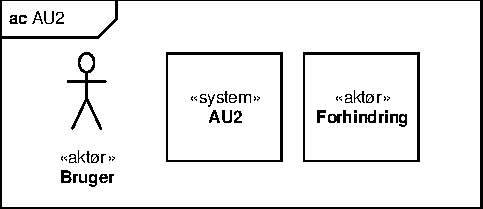
\includegraphics[width=\textwidth - 3 cm]{fig/diagrammer/ac_au2.pdf}
\caption{Skitse af hovedmenuen på brugerfladen.}
\label{fig:aktor_kontekst}
\end{figure}

\section{Aktørbeskrivelser}
\subsubsection{Bruger - Primær Aktør}
Bruger kan:
\begin{itemize}
\item Starte og stoppe systemet 
\item Styre bilen over et netværk.
\item Deaktivere og aktivere anti-kollisionssystem.
\item (Vælge forskellige grader af anti-kollisionssystem??)
% Der menes her, at det skal være muligt at vælge imellem bremse- og styreting skal være aktivt eller ej.
\end{itemize}

\section{Funktionelle krav}
Systemet\ldots
\begin{enumerate}\itemsep1pt \parskip0pt \parsep0pt
	\item \ldots  \emph{Skal} kunne køre frem og tilbage.
	\item \ldots  \emph{Skal} kunne dreje.
	\item \ldots  \emph{Skal} have hastighedsregulering.
	\item \ldots  \emph{Skal} give Bruger mulighed for at begrænse maksimumshastighed.
	\item \ldots  \emph{Skal} give Bruger mulighed for manuel styring.
	\item \ldots  \emph{Skal} via Wi-Fi kommunikere mellem bil og computer.
	\item \ldots  \emph{Skal} kunne identificere forhindringer foran og bag bilen.
	\item \ldots  \emph{Skal} indholde et anti-kollisionssystem bestående af afstandssensorer.
	\item \ldots  \emph{Skal} via. anti-kollisionssystemet kunne undvige og/eller stoppe før kollision.
	\item \ldots  \emph{Bør} give Bruger mulighed for at aktivere/deaktivere anti-kollisionssystemet på bilen.
	\item \ldots  \emph{Bør} indeholde en batteriniveau-indikator.
	\item \ldots  \emph{Bør} give Bruger mulighed for valg af indstillinger for anti-kollisionssystemet.
	\item \ldots  \emph{Kan} indeholde et kamera til at streame video.
\end{enumerate}

\section{Ikke-funktionelle krav}
\begin{enumerate}
	\item Bilens maksimumshastighed uden begrænsning er 20km/t $\pm$ 5\% %TODO Passer denne?
	\item Bilens bremselængde ved maksimumshastighed uden begrænsning må ikke overstige 1 m. %TODO Passer denne?
	\item Bilen skal kunne accelerere fra 0 km/t til maksimumshastighed uden begrænsning på højest 6 s. %TODO Passer denne?
	\item Forsinkelse fra brugerinput til at bilen reagerer må ikke overstige 50ms. %TODO Passer denne?
	\item Afstandssensorerne skal kunne identificere en forhindring på en maksimal afstand af 6 m. %TODO Passer denne?
	%TODO EMC?? Spørg vejleder.
	\item Mister bilen kommunikationen med computeren i mere end 50ms, stopper bilen automatisk. %#namepun
	
\end{enumerate}